SKA \textcolor{teal}{(Quizas me pase de quisquilloso, pero aqui agnadiria el 
"telescope".)} will be the world's largest radio-telescope. It will be located 
in two different
geographical areas: South Africa and Australia/New Zealand. It will be
constructed in different phases: SKA1 (phase 1 2018-2023) and SKA2 (phase 2
2023-2033). The development will be deployed using two different pathfinders
existing on each place (MeerKAT in South Africa [REF] and ASKAP in Australia [REF]).  
SKA1 starts in 2018 and it is intended to provide \textcolor{red}{provide o cover?} the ~10\% of
the total area at low and mid frequencies by 2023. SKA2 has
the goal to get the full array working at low and mid frequencies by 2030.
However, this timing schedule is not the final decision and some changes could
be applied for future versions \textcolor{red}{yo quitar�a esta frase} 
\textcolor{teal}{Tienes mas razon que un santo}.

There will be two different SKA facility locations depending on the frequency
range for the sky observations. A common factor in both of them, is the high l
evel of synchronisation accuracy due to the huge number of antennas needed.
More information can be found in  \cite{ska:baseline_description_v2}. Under
this context and as \cite{HUANG201727} suggests, the computer network in
astrophysics science is one of the most important elements and determines key
aspects such as system performance.

\subsection{SKA Telescope Network} \label{subsec:ska-telescope}

The SKA Telescope uses different types of networks to guarantee a proper
operation of the infrastructure. These networks are described briefly in
Figure \ref{fig:ska_net_arch1}. The design of the network corresponds to the
Signal and Data Transport (SaDT) element \cite{ska:sadt_website} and it
includes all the necessary hardware and software for the transmission of data and
information between the elements of SKA. SADT also contains details about
the provision of timing which is critical for interferometry.  The data network
includes the Digital Data Back-haul (DDBH) that transports signals from the
radio telescopes to the Central Signal Processor (CSP), and data products from
the CSP to the Science Data Processor (SDP) and from the SDP to the regional
SKA Data Centres. The total data rates are very high, approximately 80 Tb/s for
the DDBH links and another 80Tb/s for the CSP links \cite{ska:consortia-news}.
Also covered by the SaDT is the Monitor and Control (M\&C) that transmits and
receives monitoring and control information throughout the system and includes
the Telescope Manager, itself comprised of three logical networks: Production
Network, Engineering Network and Safety Network.

\begin{figure}[H] \centering 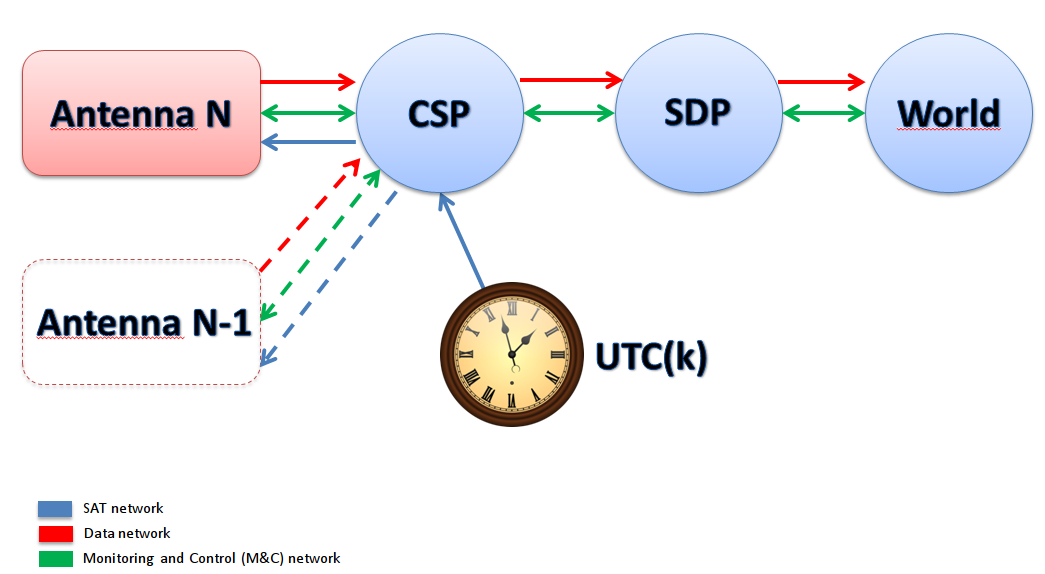
\includegraphics[scale=0.4]{img/ska_network_arch}
	\caption{The SKA Telescope network architecture is composed of three
	networks: the data network (red), the M\&C network (green) and the SAT
	network (blue). An external clock reference, UTC traceable, is provided
	to the whole Telescope elements in order of providing an unique time
	reference.} \label{fig:ska_net_arch1} \end{figure}

The final part of the SaDT is the Synchronisation and Timing (SAT) that
provides frequency and clock signals from a central clock ensemble to all
elements of the system to maintain the same phase information on all receptors, 
timing signals for data identification and time critical activities. 
In order to maintain phase coherence across the array, it is required a short-term 
timing precision of around 1 ps, while  an accuracy of 10 ns for 10 years periods 
becomes mandatory for long-term timing pulsar requirements. 
Timing is critical for the correct SKA functioning to
work as a unified large telescope using a technique known as interferometry.
This contribution focuses on the high accuracy synchronisation method used for
SKA responsible to provide a PPS signal to the critical elements. 

\FloatBarrier
\subsection{High-accuracy timing signals distribution for SKA1}
\label{subsec:ska-distribution}

As determined by SaDT, the SKA Telescope should be able to distribute a common
frequency reference to all the telescopes (\textcolor{teal}{telescopes or 
antennas??}) in order to provide a unique time reference
to register all the events with ultra-high accuracy using time-stamps. This
task is performed by the SAT element that belongs to
SaDT. The SKA timescale is maintained by the central clock ensemble for each
telescope and \textcolor{red}{will be steered to within designed limits of UTC [no se entiende]} and monitored
with respect to UTC via GNSS time transfer techniques. These clock ensembles
form the fundamental timescale for SKA and will be the basis to perform precise
measurements of pulsars and other time-dependent phenomenons. As consequence,
during this distribution, UTC refers to UTC (SKA), as realised by the central
SKA clock ensemble.  This article focuses on the solutions to distribute
the UTC time by means of PPS. This PPS signal guarantees that all the
scientific data are time-tagged using a common reference. This time reference has
high requirements coming from science that are not mandatory by other elements
of the SKA systems, such as the monitor and control network. For these other
elements, standard time transfer protocols as NTP or PTP are a feasible
solutions. For the Telescope (\textcolor{teal}{no deberia ir en minuscula?}) 
core, we illustrate that the high performance
requirements imposed by the challenging scientific goals force to provide much
more sophisticated approaches.  The PPS distribution system will be in charge
of delivering its output at the following locations: SKA1-MID with 133 dishes
connected to optical fibre links between 120-150 km and SKA1-LOW with 45
stations along 3 spiral arms connected to optical fibre links between 70-80 km.

Depending on the frequency offset scheme applied to all SKA1-MID dishes,
additional 64 endpoints may be needed in SKA1-MID. By this, the synchronization
network might be increased from 182 to 246 endpoints.  
As previously said, the SAT array general requirements for the frequency distribution is 1 ps 
while the time synchronisation and time-stamp requirements reaches 10 ns, being mandatory for the whole network.
SaDT uses different mechanisms to achieve frequency dissemination and PPS distribution goals. 
Our contribution  focuses on describing a  suitable candidate solution for the PPS
distribution system, whilst the related work only considers the second requirement. Note that
a complete description of the SKA network elements and topology is out of the
scope of this contribution and only the requirements needed are presented to
properly understand the need of the solution here developed.
\textcolor{red}{Due to the fact that the main clock also consumes part of this, it translates
into PPS-distribution time requirement of 5 ns. The error here includes PPS
distribution, delay centre precision, Dish timing transport and time-stamping
errors and should be distributed on the different elements of the system that
rely on the network topology that determine the number of hops. [no se entiende]} Based on
current SAT network topology, the target specification for the elements of the
PPS distribution system provides them an average time better than 2 ns. This is
a quite challenging goal not only because it imposes a high accuracy
synchronisation requirement but also for the environmental conditions of the 
installation that must be taken into account. \textcolor{teal}{Me resulta raro 
soltar eso asi... No se si es cosa mia pero para la primera parte de la frase 
ya la has argumentado correctamente mientras que para la segunda no, dado que 
eso viene luego. Para mi queda raro, o todo antes o todo despues.}
SKA1 uses aerial optical fibre networks that are
significantly affected by the large temperature excursion during operation,
presenting variations of more than 20º in desert locations, such as South Africa and
Australia. Furthermore, outdoor wind velocities during normal operation
could achieve up to 40 km/h, making fibres oscillate and changing their
length, forcing to develop a compensation mechanism on real-time during execution or \textcolor{red}{averaged
them out. ???} \textcolor{teal}{Forcing es demasiado severo, de hecho, tras las 
pruebas de este paper se deja ver que lo de la temperatura tampoco es tanto 
problema.}

Next section provides the description of the authors' proposed solution for the 
SKA Telescope\textcolor{teal}{'s} PPS distribution system. 


